\section{T-FINANCE AND WEIBO SOURCE SENSITIVITY}
\label{app:extensions}
\paragraph{Protocol and acquisition.}
The T-Finance protocol was saved before loading model outcomes. We downloaded the T-Finance and Weibo members of the official GADBench archive~\citep{tang2023gadbench}, verified ZIP CRC and SHA-256, and retained their distributed binary labels and numerical features without relabeling. Raw adjacency is symmetrized, binarized, and stripped of self loops. T-Finance has 39,357 nodes, 10 features, 1,803 anomalous labels and 21,222,543 undirected edges. GADBench Weibo has 8,405 nodes, 400 features, 868 anomalous labels and 377,271 undirected edges. Original GADBench train/validation/test masks are not used; we apply the same uniform 10\% training-panel design as the other controls.

\paragraph{Weibo provenance.}
The actual official PyGOD file has 347 anomalous labels despite its README's stated 868. A fresh download is byte-identical to our raw input, and the cached labels equal those distributed labels. The separately distributed GADBench file has 868 anomalous labels. The two raw feature matrices agree entrywise and their symmetrized, loop-free adjacency matrices agree. Two nodes share identical features and symmetric neighborhoods, so external node identities are not established uniquely from those arrays alone. The existing PyGOD processed cache standardizes features; this source extension preserves GADBench's raw distributed features. We therefore report a source sensitivity, not a claim that every numerical difference isolates label changes alone. PyGOD and GADBench outcomes are never pooled.

The raw GADBench Weibo SHA-256 is
\texttt{111402a2cb3b6a10\allowbreak ec586e96122da809\allowbreak d62bfe3617add07cb\allowbreak 006de53fc109f05};
T-Finance is
\texttt{8f3b05272703220b\allowbreak b3248b0caac92e91\allowbreak 7c7524704094c02f\allowbreak 802b400026ed1d38}.
The machine-readable provenance includes full hashes, upstream commit, download ranges, actual field shapes and processed-graph hashes.

\paragraph{Training and evaluation.}
For each graph, fit ten attribute-only and ten graph-feature histogram-gradient-boosting scorers with the fixed settings in Appendix~\ref{app:supervised}. T-Finance has 3,936 training labels and GADBench Weibo has 840. Training labels never re-enter calibration or testing. All calculations use sparse adjacency and CPU training. Each extension retains five test splits, three label-revelation fractions, nine removal fractions, two matched rules and fifty calibration repetitions: 270,000 evaluations per source. The Weibo sensitivity uses the earlier Weibo RNG namespace, while T-Finance uses a new dataset index; class-stratified test identities can change when source labels differ. All results, including abstentions and unsuccessful contrasts, are retained. Neither score direction nor hyperparameters are selected using these outcomes.

\begin{table*}[t]\centering\small
\caption{Prespecified 20\%-removal comparison with half of non-test labels revealed. FDP/power pairs average all outcomes; ranking metrics average ten training seeds. Full curves follow.}
\begin{tabular}{llrrrr}\toprule Graph & Score & AUROC & AP & Exposure FDP/power & Random FDP/power\\\midrule
T-Finance & Attributes & $0.940$ & $0.794$ & $0.127/0.668$ & $0.093/0.650$ \\
T-Finance & Graph features & $0.962$ & $0.880$ & $0.191/0.830$ & $0.095/0.789$ \\
Weibo (GADBench) & Attributes & $0.982$ & $0.899$ & $0.184/0.783$ & $0.094/0.663$ \\
Weibo (GADBench) & Graph features & $0.993$ & $0.954$ & $0.286/0.973$ & $0.091/0.844$ \\
\bottomrule\end{tabular}\end{table*}

\begin{figure*}[t]\centering
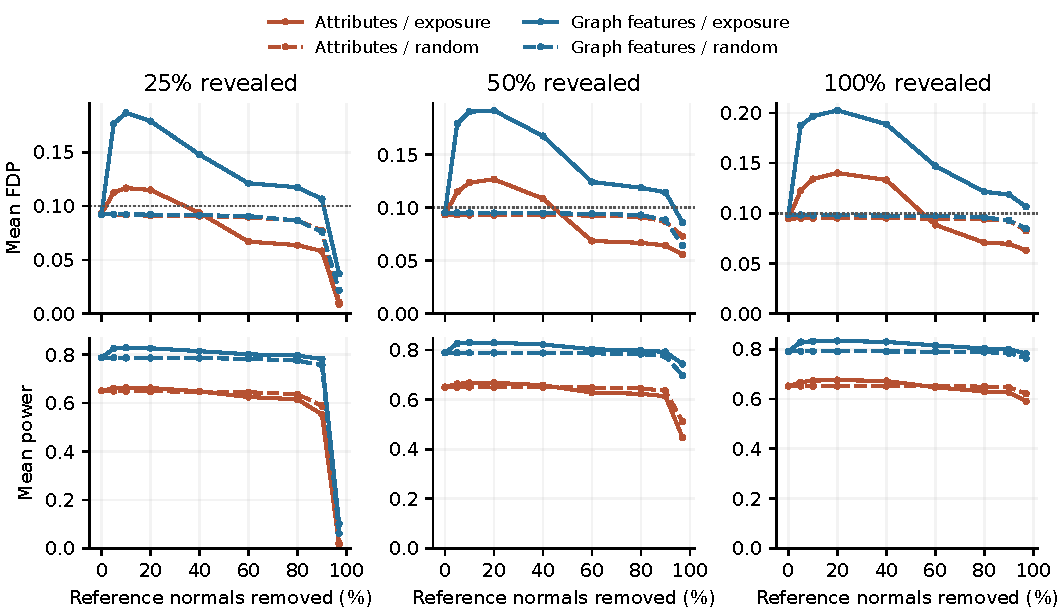
\includegraphics[width=\textwidth]{extension_dose_tfinance.pdf}
\caption{T-Finance: complete prespecified removal sweep. Both scorers, all nine removal fractions and all three revelation fractions are shown. Solid lines use exposure removal; dashed lines use equally sized random references. Means retain every abstention and average ten training-seed means.}
\end{figure*}

\begin{figure*}[t]\centering
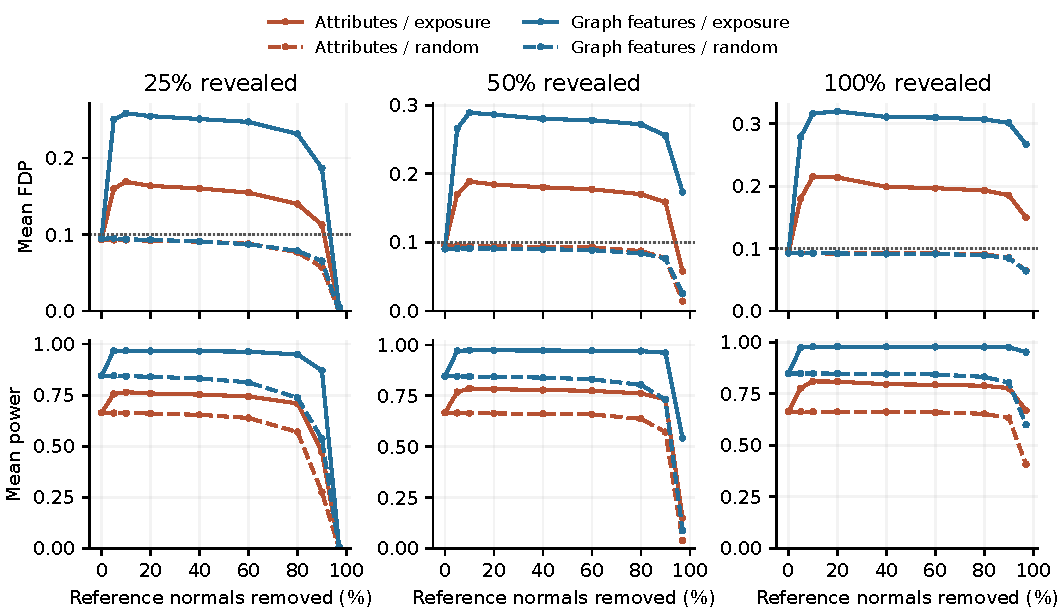
\includegraphics[width=\textwidth]{extension_dose_weibo_gadbench.pdf}
\caption{Weibo (GADBench): complete prespecified removal sweep. Both scorers, all nine removal fractions and all three revelation fractions are shown. Solid lines use exposure removal; dashed lines use equally sized random references. Means retain every abstention and average ten training-seed means.}
\end{figure*}